\title{WiMAX Measurements \\
{\small CS707 Assignment 1}
}
\author{
    Robert Jellinek, Siva Ramasubramanian \\
    University of Wisconsin-Madison \\
    \{jellinek, sivas\}@cs.wisc.edu
}
\date{\today}

\documentclass[12pt]{article}
\usepackage[hyphens]{url}
\usepackage[margin=1.5in]{geometry}
\usepackage{graphics,epsfig}

\begin{document}
\maketitle

%\begin{abstract}
%\end{abstract}

\section{Introduction}
For this project, our goal was to take 20 measurements---10 line-of-sight (LOS)
and 10 non-line-of-sight (NLOS)---of statistics describing the quality of the
channel between the WiMAX station at the top of the Computer Sciences building.
Our goal was to record a set of measurements that was diverse enough to use to
build a model that takes a set of GPS coordinates as parameters and returns the
predicted signal strength. That is, we hypothesize that our signal-strength
measurements, when used under an appropriate model, can predict signal strength
at other locations.

\section{Methodology} We collected our measurements by walking from point to
point, arranging the WiMAX dongle such that it faced the access point (AP)
antenna on the top of the Computer Sciences building, and running a number of
tests five times each at each location. We made sure that we did not stand
between our WiMAX antenna and the AP in order to avoid interfering with (i.e.
weakening) the signal.  We used the WiMAX card's web-based management interface
tool to collect data on RSSI and CINR. We then used \textit{iperf} to record
data on the card's uplink speed, and \textit{speedtest.net} to measure the
link's downlink speed. We also recorded time, and used the Locus app on an
Android phone to record and plot the GPS coordinates of our measurements.

Our LOS data was captured by walking up Monroe St., making sure the WiMAX
antenna was visible from our position, and performing the tests mentioned above.
For our NLOS tests, we walked some distance from Monroe St. such that our
position obscured our view of the WiMAX antenna. While we attempted to diversify
our range of locations, dusk and impending rain forced us to remain close to
Monroe St. The final two LOS and final three NLOS data points were recorded one
day after the other measurements. Measurements are visible in Figure
\ref{fig:locations}.

%% TODO include location plots here
\begin{figure}[t]
\center
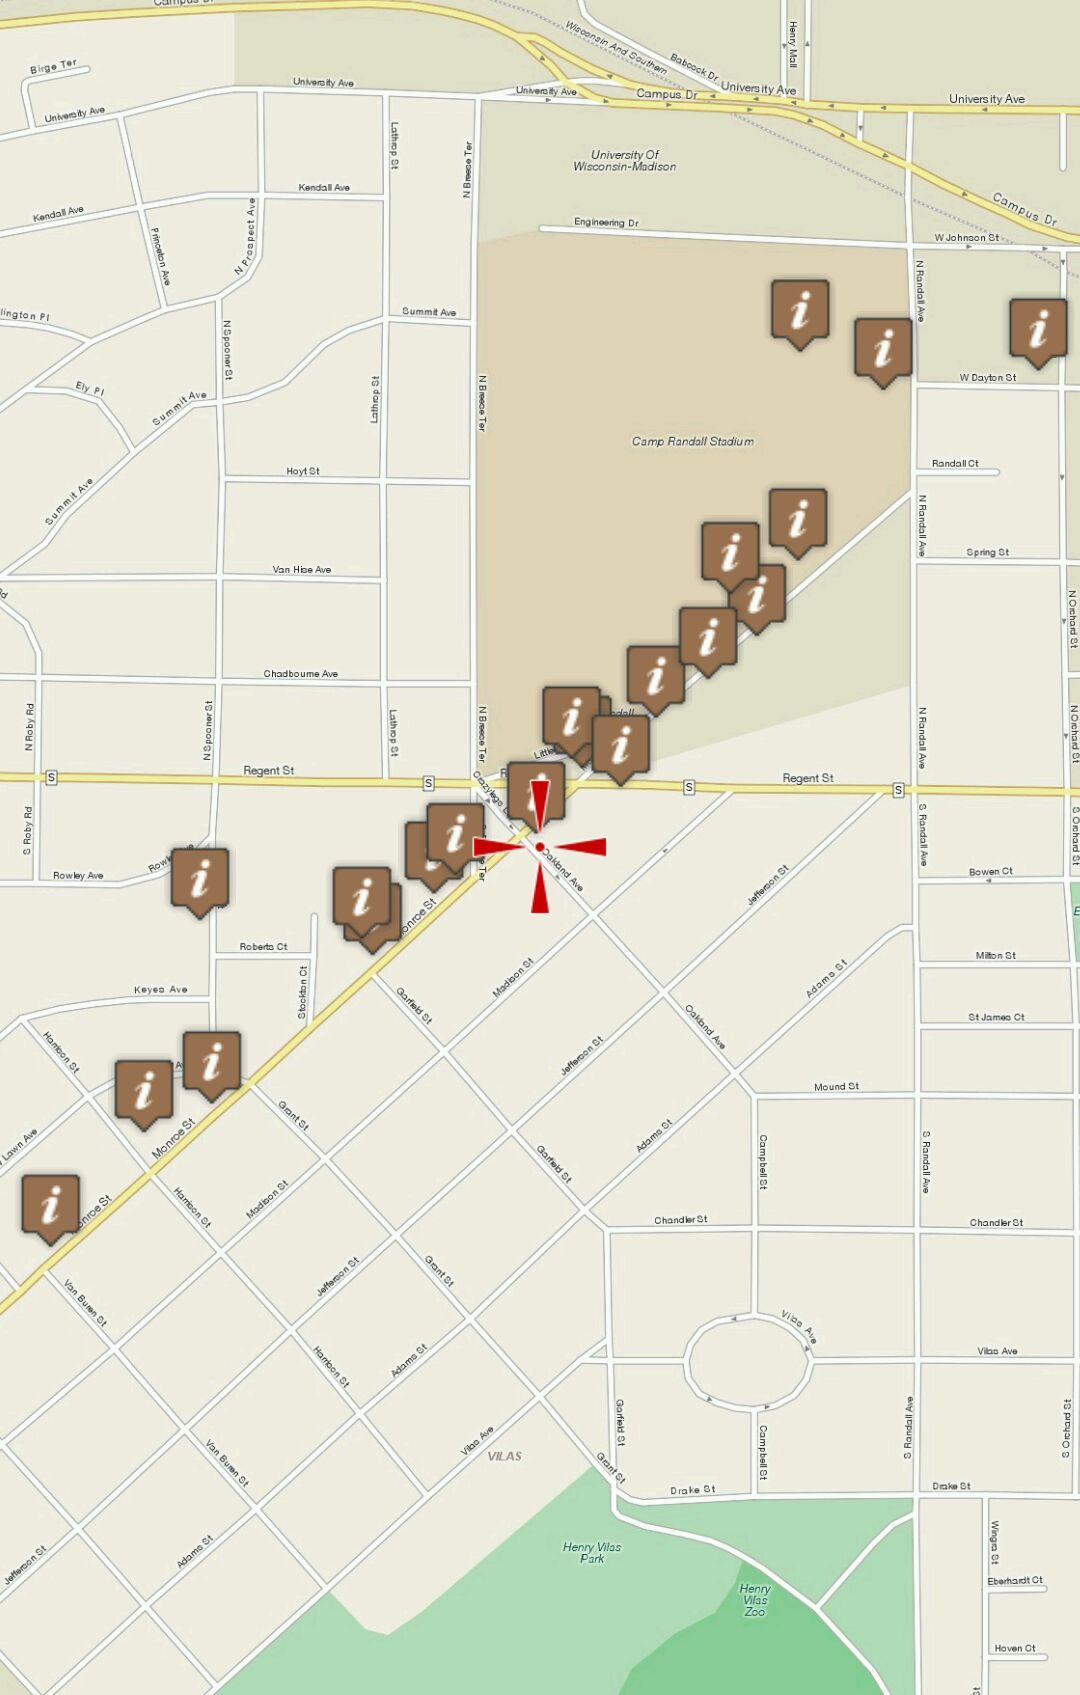
\includegraphics[width=.5\linewidth]{locations}
\caption{Locations of our LOS and NLOS measurements.}
\label{fig:locations}
\end{figure}

\section{Model}
Our model depends on handling LOS and NLOS measurements separately, since even
though two sampling locations can be geographically very close, the introduction
of obstacles in the signal path can have a substantial effect on signal
strength.

\section{Results}
\section{Conclusion}

%\bibliographystyle{abbrv}
%\bibliography{biblio}

\end{document}
